\documentclass[10pt, a4paper]{report}
\usepackage{graphicx}
\usepackage{multicol}
\usepackage{tabularx}
\usepackage[toc]{appendix}
\usepackage{amssymb}
\usepackage{amsmath}
\usepackage{datetime}
\usepackage{amsthm}
\usepackage{tikz}
\usetikzlibrary{arrows.meta}
\usepackage{algorithm}
\usepackage{algpseudocode}
\usepackage{pdfpages}

\theoremstyle{definition}
\newtheorem{definition}{Definition}

\newtheorem{theorem}{Theorem}

\newcommand{\reporttitle}{Explaining Optimisation Solvers}
\newcommand{\reportauthor}{Myles Lee}
\newcommand{\supervisor}{Dr. Kristijonas Cyras\\Prof. Francesca Toni}
\newcommand{\reporttype}{MEng. Individual Project}
\newcommand{\linespace}{\vspace*{\baselineskip}\\}
\newcommand{\pair}[2]{\langle{#1},{#2}\rangle}
\tikzstyle{file} = [draw, inner sep=10pt]
\tikzstyle{node} = [draw, circle, inner sep=5pt]
\tikzstyle{arrow} = [-{Stealth[scale=2]}]

\makeatletter
\newcommand{\incircbin}{\mathpalette\@incircbin}
\newcommand\@incircbin[2]{\mathbin{\ooalign{\hidewidth$#1#2$\hidewidth\crcr$#1\bigcirc$}}}

\begin{document}
	
	\begin{titlepage}
	\newdateformat{monthyeardate}{\monthname[\THEMONTH] \THEYEAR}
	
	\noindent
\includegraphics[width=7cm]{./figures/imperial_logo}
	
	\Large\centering
	
	\vspace*{3\baselineskip}	
	\textsc{\LARGE \reporttype}
	
	\vspace*{\baselineskip}	
	\textsc{Imperial College of Science, Technology and Medicine}

	\vspace*{\baselineskip}	
	\textsc{Department of Computing}


	\setlength{\parindent}{0pt}
	
	\setlength{\parskip}{0pt}

	\rule{\linewidth}{0.4pt}\vspace*{\baselineskip}

	{\huge\bfseries\reporttitle}
	\rule{\linewidth}{0.4pt}

	Draft Final Report

	\begin{multicols}{2}
		\begin{flushleft}
			\emph{Author:}
			
			\reportauthor
		\end{flushleft}
		\columnbreak
		\begin{flushright}
			\emph{Supervisors:}
			
			\supervisor	
			\linespace
			\emph{Second Marker:}
			
			\marker
		\end{flushright}			
	\end{multicols}
	
	\vspace*{\stretch{1}}
	
	% fix this to June 2019 on submission
	\monthyeardate\today
	
	\vspace*{\stretch{1}}
	
\end{titlepage}

	
	\begin{abstract}
		Scheduling arises in many decision processes and has a wide range of practical applications, such as in healthcare. Scheduling problems are mathematically modelled, where optimisers find solutions to large scheduling problems quickly. Problems and solutions are often complex with non-accessible formulations, resulting in users interpreting solvers and solutions as black-boxes. Users require a means to understand why a schedule is reasonable, which is hindered by black-box interpretations.
\linespace
We build an argumentation-supported tool, namely \emph{\toolname} that explains any makespan schedule easily with clarity. We will explore practical considerations of applied argumentation to makespan scheduling and theoretical generalisations of argumentation, as in interval scheduling.
	\end{abstract}
	
	\pagenumbering{roman}
	\tableofcontents 
	 
	\cleardoublepage
	\pagenumbering{arabic}

	\chapter{Introduction}
	
\section{Motivation}

Scheduling arises in countless decision processes and its abstract nature results in a wide range of practical applications, such as in healthcare \cite{sanr}. Scheduling problems are accurately modelled in mathematics, hence scheduling is often interpreted as a class of mathematical optimisation problems. With many mature and developed optimisation solvers \cite{clp}, solvers can find solutions to large scheduling problems quickly, which would have been impractical using manual optimisation techniques. However, solver scalability and efficiency often leads to complex algorithms. Such complexity combined with mathematical formulations of scheduling, result in users interpreting solvers and solutions as black-boxes. Therefore, decision making of schedules are often not transparent.
\linespace
Transparency of decision making is important. Users require a means to understand why a schedule, whether a solution of a solver or not, is reasonable given a context. For example, hospital managers may seek understanding about the efficiency of their staff and resources. Schedules may need to be robust to unpredictable changes in staff and resources, such as a nurse being unavailable to attend patients due to a personal reasons. In other settings, schedules may need to minimise the number of staff to maximise profits while fulfilling all staff and patients requirements.
\linespace
Explanations are vital in communication for understanding. With many possible schedules, and many variations of scheduling problems \cite{sta}, it is impractical to manually-craft explanations for every schedule of every variation. This motivates a tool to generate clear explanations.

\section{Objectives}

The first main objective is to devise and implement a tool that explains an solver's scheduling solutions by human-understandable means, and allows the user to interact with the solver in a human-friendly manner. By using the explanation methodology outlined using argumentation \cite{aes}, the user can easier understand scheduling in a practical environments such as nurse rostering and dialysis scheduling. Hence, analysis of such methodology important to understand the applicability of argumentation in practical settings.
\linespace
The second main objectives is to extend the theorical or practical capabilities of argumentation for scheduilng. Extensions may include interval scheduling, shop scheduling and job-dependent scheduling.

\section{Challenges}

A tool satisfying such objectives are subjected solving the challenges:
\begin{enumerate}
	\item\textbf{Accessibility:} Explanations generated from this tool are required to be accessible to people without domain-specific knowledge of optimisation or argumentation. The tool should be accessible to computer novices.
	\item\textbf{Applicability:} Explanations should relate to schedules. The tool should generate clear explanations promptly.
	\item\textbf{Knowledge transfer:} Explanations are constructed using knowledge structures, commonly represented using natural languages or diagrams. A challenge would be to effectively explore the usefulness of using natural languages compared to diagrams.
	\item\textbf{Trust:} Users of the tool need to be confident that the explanations generated are true. This requires correctness of algorithms implemented.
	\item\textbf{Background:} Explanable planning is relatively new research area compared to optimisation \cite{pe}.
\end{enumerate}

\section{Contributions}

The main contributions of this report are listed below:
\begin{itemize}
	\item A new tool \emph{Argumentative Explainable Scheduler} that implements the concepts behind using argumentation for optimisation for makeshift scheduling.
	\item Theorical extensions to makeshift scheduling including interval scheduling.
	\item Algorithmic optimisations of argumentation with scheduling.
	\item A dicussion on applicability of argumentation models against various scheduilng models.
\end{itemize}

	\chapter{Background}

\section{Optimisation}

Optimisation is the process to finding the optimal decision with respect to constraints given a set of possible decisions. The optimal decision is measured by a cost function, that typically determines a numerical value representing how good a decision is. The problem is to either find the optimal decision, either as a minima or maxima using systematic methods. Applications of optimisation occur in many practical situations such as in engineering, manufacturing, science. In engineering applications, accurate modelling of a problem may require discrete decisions and non-linear relationships, resulting in difficulty in finding arbitrary optimal decisions. The wide range of applications of optimisation result in  many fields of optimisation, where in this project we look at MILP.
\begin{center}
	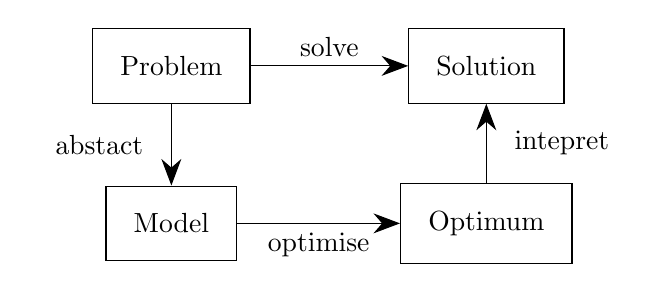
\begin{tikzpicture}
		\node[file](problem) at (0, 2){Problem};
		\node[file](model) at (0, 0){Model};
		\node[file](solution) at (4, 2){Solution};
		\node[file](optimum) at (4, 0){Optimum};
		\draw[arrow](problem) -- node [above] {solve} (solution);
		\draw[arrow](problem) -- node [left, inner sep=10pt] {abstact} (model);
		\draw[arrow](model) -- node [below] {optimise} (optimum);
		\draw[arrow](optimum) -- node [right, inner sep=10pt] {intepret} (solution);
	\end{tikzpicture}
\end{center}
Real-life problems need to be modelled to be optimised. Problems are formulated using constraints and a cost function. Consider the following linear programming example. A person want to sell some drinks. Each unit of hot chocolate requires 1 litre of milk and 3 bars of chocolate. Each unit of milkshake requires 1 litre of milk and 2 bars of chocolate. The person only has 5 units of milk and 12 bars of chocolate. The person sells a unit of hot chocolate for £6 and a unit of milkshake for £5. What is the best strategy for maximising profit given that all units produced are sold? The problem is abstracted as follows. Let $x$ and $y$ be the number of hot chocolates and milkshakes produced.
\begin{align*}
	\max_{x,y}\ &6x+5y&\text{subject to:}\\
	&x+y\leq 5&\text{milk resource constraint}\\
	&3x+2y\leq 12&\text{chocolate resource constraint}\\
	&x,y\geq 0&\text{non-negative constraints}\\
	&x,y\in\mathbb{N}&\text{whole units only}\\
\end{align*}
The problem is sufficiently small to be solved by inspection, but may also be solved using graphical methods or a simplex algorithm. The optimum is $x^*=2$ and $y^*=3$, which is interpreted as that the best strategy is producing 2 units of hot chocolate and 3 units of milkshake.
\linespace
In non-linear optimisation problems, finding global optimums in not trivial. For gradient-based and local-search algorithms, estimated solutions can return local optimums. This is typically not favoured however for large problems, finding global optimums have non-polynomial complexity. In context of the project, it would not be feasible to compute an explanation in polynomial time.

\subsection{Makeshift Scheduling}

The simplistic definition of makeshift scheduling gives a good foundation for experimenting with argumentation. Makeshift schedules are defined by a $m\in\mathbb{N}$ independent machines and $n\in\mathbb{N}$ independent jobs \cite{sa}. Let $\mathcal{M}=\{1,...,m\}$ be the set of machines and $\mathcal{J}=\{1,...,n\}$ be the set of jobs. Each job $i\in\mathcal{J}$, has an associated processing time $p_i\in\mathbb{R}_{\geq 0}$. All processing times are collectively denoted by a vector $\mathbf{p}$. A machine can only execute at most one job at any time. For a feasible schedule, each job is assigned to a machine non-preemptively. For some $i\in\mathcal{M}$, let $C_i$ be the completion time of the $i^\text{th}$ machine. Let $C_{\max}$ be the total completion time. Let $\mathbf{x}\in\{0,1\}^{m\times n}$ be the assignment matrix that allocates jobs to machines. Formally, makeshift schedules are modelled as an optimisation problem:
\begin{align*}
	\min_{C_{\max},\mathbf{C},\mathbf{x}}&C_{\max}&\text{ subject to:}\\
	\forall i\in\mathcal{M}.\ &C_{\max}\geq C_i\\
	\forall i\in\mathcal{M}.\ &C_i=\sum_{j\in\mathcal{J}}x_{i,j}\cdot p_j\\
	\forall j\in\mathcal{J}.\ &\sum_{j\in\mathcal{J}}x_{i,j}=1\\
	\forall i\in\mathcal{M},\ \forall j\in\mathcal{J}.\ &x_{i,j}\in\{0,1\}
\end{align*}

\begin{definition}
	A schedule $S$ is defined by its assignment matrix $\mathbf{x}$ such that $S=\mathbf{x}$.
\end{definition}

\begin{definition}
	A schedule $S$ is optimal iff $S$ achieves the minimal total completion time.
\end{definition}


\begin{definition}
	A machine $i\in\mathcal{M}$ is critical iff $C_i=C_{max}$.
\end{definition}

\begin{definition}
	A job $j\in\mathcal{J}$ is critical iff $j$ is allocated to a critical machine $i\in\mathcal{M}$ such that $x_{i,j}=1$.
\end{definition}

\begin{definition}
	A schedule satisfies the single exchange property (SEP) iff for any critical machine and any machine $i,i'\in\mathcal{M}$ and for all critical jobs $j\in\mathcal{J}$, $C_i-C_{i'}\leq p_j$
\end{definition}

\begin{definition}
	A schedule satisfies the pairwise exchange property (PEP) iff for any critical job and any job $j,j'\in\mathcal{J}$, if $p_j>p_{j'}$, then $C_i+p_{j'}\leq C_{i'}+p_j$.
\end{definition}

\begin{definition}
	A schedule $S$ is efficient iff $S$ satisfies SEP and PEP.
\end{definition}

\begin{theorem}
	Schedule efficiency is a necessary condition for optimality.
\end{theorem}

Makeshift schedules are often represented using cascade charts. The first and second chart shows an inefficient schedule and efficient schedule respectively where $m=4$ and $n=12$.

\begin{center}
	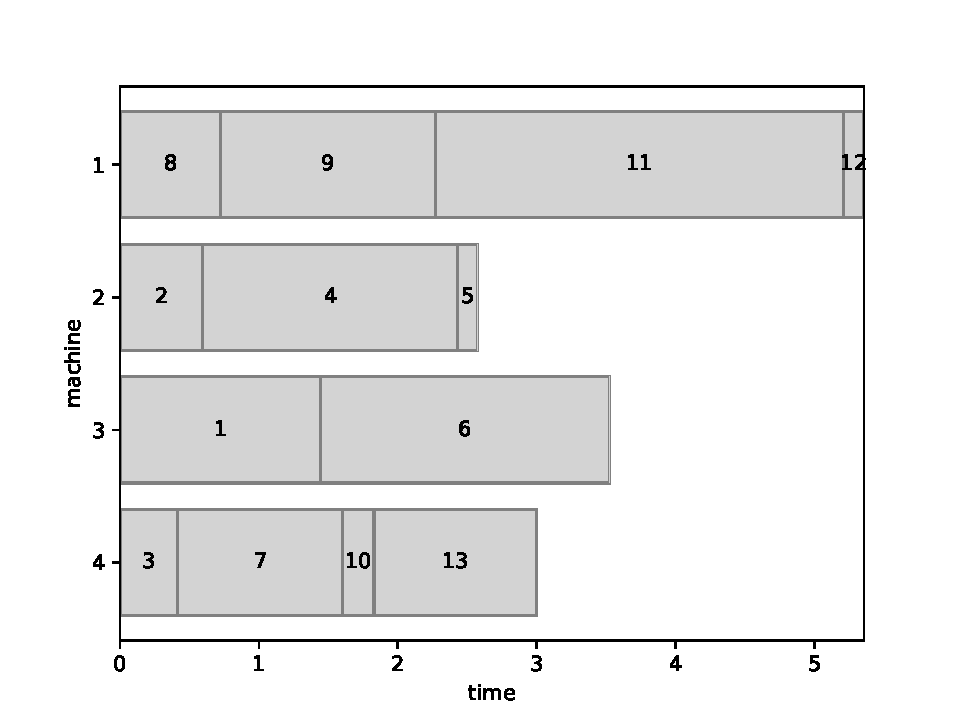
\includegraphics[width=.6\linewidth]{figures/makeshift1.pdf}
\end{center}

\begin{center}
	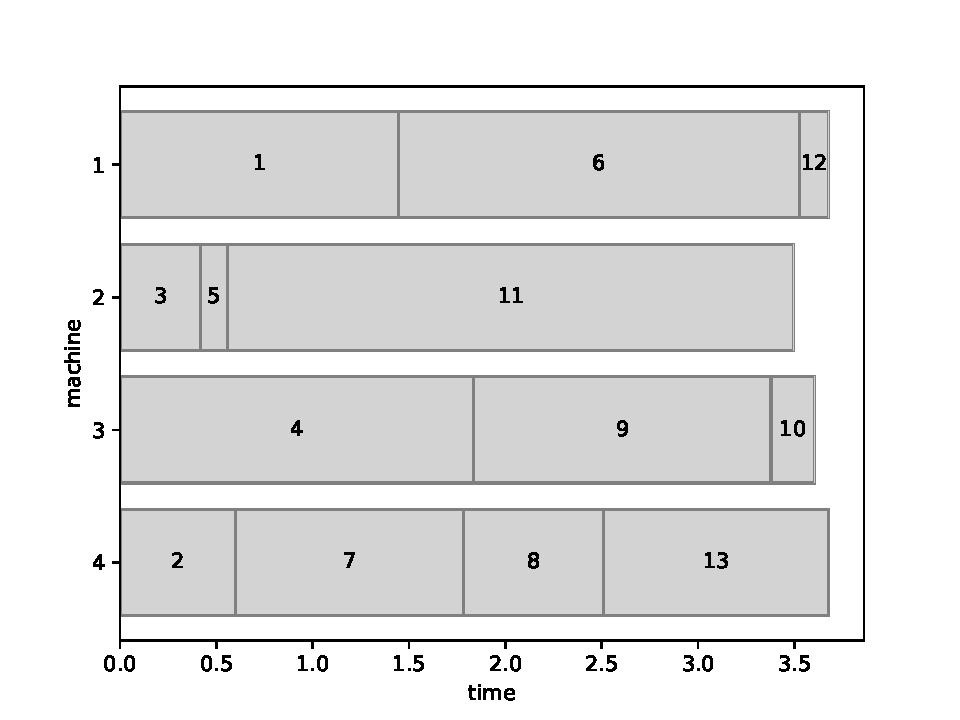
\includegraphics[width=.6\linewidth]{figures/makeshift2.pdf}	
\end{center}

\subsection{User Fixed Decisions}

To accommodate practical applications of makeshift schedules, user positive and negative fixed decisions are introduced as an extension. In a hospital setting, positive fixed decisions capture patients exclusively allocated to a nurse while negative fixed decisions capture unavailable or incompatible nurses and patients. Let $D^-,D^+\subseteq\mathcal{M}\times\mathcal{J}$ be the negative and positive fixed decisions respectively. Let $D$ be the fixed decisions such that $D=(D^-,D^+)$.

\begin{definition}
	A schedule $S$ satisfies $D$ iff $\forall(i,j)\in D^-.\ x_{i,j}=0$ and $\forall (i,j)\in D^+.\ x_{i,j}=1$.
\end{definition}

\begin{definition}
	A fixed decision $D$ is satisfiable iff there exists a schedule $S$ such that $S$ satisfies $D$. 
\end{definition}

\begin{theorem}
	A fixed decision $D$ is unsatisfiable iff if the following necessary and sufficient conditions hold:
	\begin{itemize}
		\item$D^+$ and $D^-$ are disjoint.
		\item$\forall(i,j),(i',j')\in D^+.\ i=i'\lor j\neq j'$
		\item$\forall j\in\mathcal{J}.\ \exists i\in\mathcal{M}.\ (i,j)\not\in D^-$
	\end{itemize}
\end{theorem}

The relaxed definition of $D$ allows $D$ to be unsatisfiable, which is not permitted in previous work \cite{aes}. This relaxation accomdates for poorly-formulated user problems, allowing explanations over validation of user input, in a practical setting.

\subsection{Interval Scheduling}

...

\section{Argumentation}

Argumentation is a method to understand and evaluate reasons for and against potential conclusions. Argumentation is useful in resolving conflicts, clarifying incomplete information and most importantly, with respect to this project, explanations. The precise definition of an argument varies on the literature, however it is commonly agreed that arguments can attack or support other arguments. For an argument $\alpha$ to attack an argument $\beta$, $\alpha$ may critically challenge $\beta$ such that acceptability of $\beta$ is doubted \cite{at}. This may be to question one of $\beta$'s premises, by proposing a counter-example. For example, consider an scenario whether to sleep. Let $\alpha$ be ``I want to sleep", $\beta$ be ``I have work to do" and $\gamma$ be ``I can work tomorrow". Using human intuition, we can derive that $\gamma$ attacks $\beta$ and $\beta$ attacks $\alpha$. This is represented graphically below.

\begin{center}
	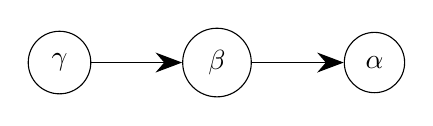
\begin{tikzpicture}
		\node[node](gamma) at (0, 0){$\gamma$};
		\node[node](beta) at (2, 0){$\beta$};
		\node[node](alpha) at (4, 0){$\alpha$};
		\draw[arrow](gamma) -- (beta);
		\draw[arrow](beta) -- (alpha);
	\end{tikzpicture}
\end{center}

If we conclude $\alpha$ to be acceptable, then we must not accept $\beta$. Accepting two arguments with conflicts can be interpreted as a contradiction or hypocritical. Hence, argumentation theory have measures of acceptable extensions, to decide whether some set of arguments are acceptable in some notion, with respect to different intuitions. This motivates to use abstract argumentation frameworks.\linespace
Note that this example uses implicit background knowledge, also known as enthymemes. In this scenario, one cannot sleep and work at the same time. To our advantage, argumentation is applied to well-defined scheduling problems, so enthymemes are inapplicable in this project.

\subsection{Abstract Argumentation Frameworks}

An abstract argumentation framework (AAF) models the relation of attacks between arguments \cite{aa}. Formally, an AAF is a directed graph $(Args,\rightsquigarrow)$ where $Args$ is the set of arguments and $\rightsquigarrow$ is a binary relation over $Args$. For $a,b\in Args$, $a$ attacks $b$ iff $a\rightsquigarrow b$. Attacks are extended over sets of arguments, where $A\subseteq Args\rightsquigarrow b\in Args$ iff $\exists a\in A.\ a\rightsquigarrow b$. An extension $E$ is a subset of $Args$.

\begin{definition}
	An extension $E$ is conflict-free iff $\forall a,b\in E.\ a\not\rightsquigarrow\ b$.
\end{definition}

\begin{definition}
	An extension $E$ is stable iff $E$ is conflict-free and
	
	$\forall a\in Args\backslash E.\ E\rightsquigarrow a$
\end{definition}

\begin{center}
	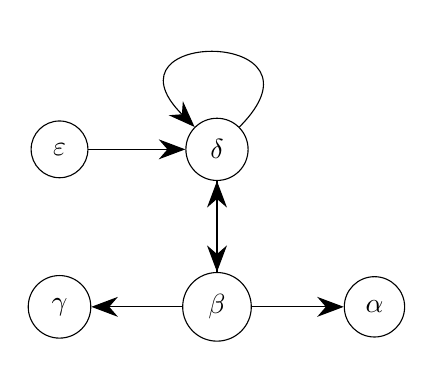
\begin{tikzpicture}
	\node[node](gamma) at (0, 0){$\gamma$};
	\node[node](beta) at (2, 0){$\beta$};
	\node[node](alpha) at (4, 0){$\alpha$};
	\node[node](delta) at (2, 2){$\delta$};
	\node[node](epsilon) at (0, 2){$\varepsilon$};
	\draw[arrow](beta) -- (alpha);
	\draw[arrow](beta) -- (gamma);
	\draw[arrow](beta) -- (delta);
	\draw[arrow](delta) -- (beta);
	\draw[arrow](delta) to [loop](delta);
	\draw[arrow](epsilon) -- (delta);
	\end{tikzpicture}
\end{center}

Consider the following example where $Args=\{\alpha,\beta,\gamma,\delta,\varepsilon\}$ and $	\rightsquigarrow=\{
\pair{\beta}{\alpha},\\
\pair{\beta}{\gamma},
\pair{\beta}{\delta},
\pair{\delta}{\beta},
\pair{\delta}{\delta},
\pair{\varepsilon}{\delta}
\}$ as illustrated above. Then the following statements hold:
\begin{itemize}
	\item $\varepsilon\rightsquigarrow\delta$.
	\item $\{\delta,\varepsilon\}\rightsquigarrow\beta$.
	\item $\{\alpha,\gamma\}$ is conflict-free but not stable.
	\item $\{\delta\}$ is not conflict-free and not stable.
	\item $\{\beta,\varepsilon\}$ is conflict-free and stable.
\end{itemize}

\section{Explanations}

asdsa

\section{Existing Tools}

asd
	\chapter{Project Plan}

\section{Milestones}

The primary objective of the project is to correctly implement the tool. The implementation is composed of multiple small milestones:

\begin{enumerate}
	\item\textbf{Solver integration:} The tool depends on an external optimisation library. External libraries are subject to licensing issues, poor interfacing and lack of clear documentation. Hence, using solvers are a significant risk.
	\item\textbf{Argumentation:} Implementation of the argumentation methodology requires through understanding of paper \cite{aes}. Background research is crucial for an efficient and extensible implementation. The paper explicitly states the definitions of required AFs, hence their construction should be trivial. However, their generated explanations from using the stability extension rely on human intuition and are not formally expressed. The paper states that for any schedule, there exists an explanation, implying that a formalism exists. This implementation would be challenging, but this is at the core of the project.
	\item\textbf{GUI:} For the tool to be accessible to computer novices, a GUI allows users to easily interact with explanations. There are many GUI tutorials for many different libraries. Choosing a GUI library will require some investigation. Creating a good user experience may be time-consuming, but this is a low risk.
\end{enumerate}

Secondary objectives would include finding opportunities to expand ArgOpt. At the time of writing, there are many future directions regarding scheduling. These include:
\begin{itemize}
	\item Modelling waiting times between jobs. This can represent delays between appointments of patients and nurses, or in general, context-switch overhead for machines.
\end{itemize}
	\chapter{Implementation}

\section{Design Decisions}

To select a programming language suitable for developing the tool, languages were compared with respect to possible challenges. The language should be compatible with popular optimisation solvers. To make efficient use of time, using an existing interface library between popular solvers is recommended. Interfaces are written for popular languages such as C++, Java and Python. Python was selected for its development speed and support for a wide range of libraries.
\linespace
There is a balance between program speed and development time. A tool written in C may be fast but time-consuming. The purpose is to demonstrate the concept of argumentation with schedules while allowing analysis of potential future directions and short-comings. Hence, the tool should be sufficiently fast to be responsive, but not necessarily fast as possible.
\linespace
There are many powerful and efficient solvers such as CPLEX [paper] and GLPK [paper]. To solver large problems, users use commercial over open-source solvers for their superior speed [paper]. However, users may not have access to a commercial solver. To accommodate users, Pyomo is used to interface to many popular solvers.
\linespace
The tool features a GUI to aid its accessibility. Users such as hospital managers can often use a suitably-designed GUI without training of the tool. In practice, a GUI is easier to demonstrate than a CLI.

\section{Structure}

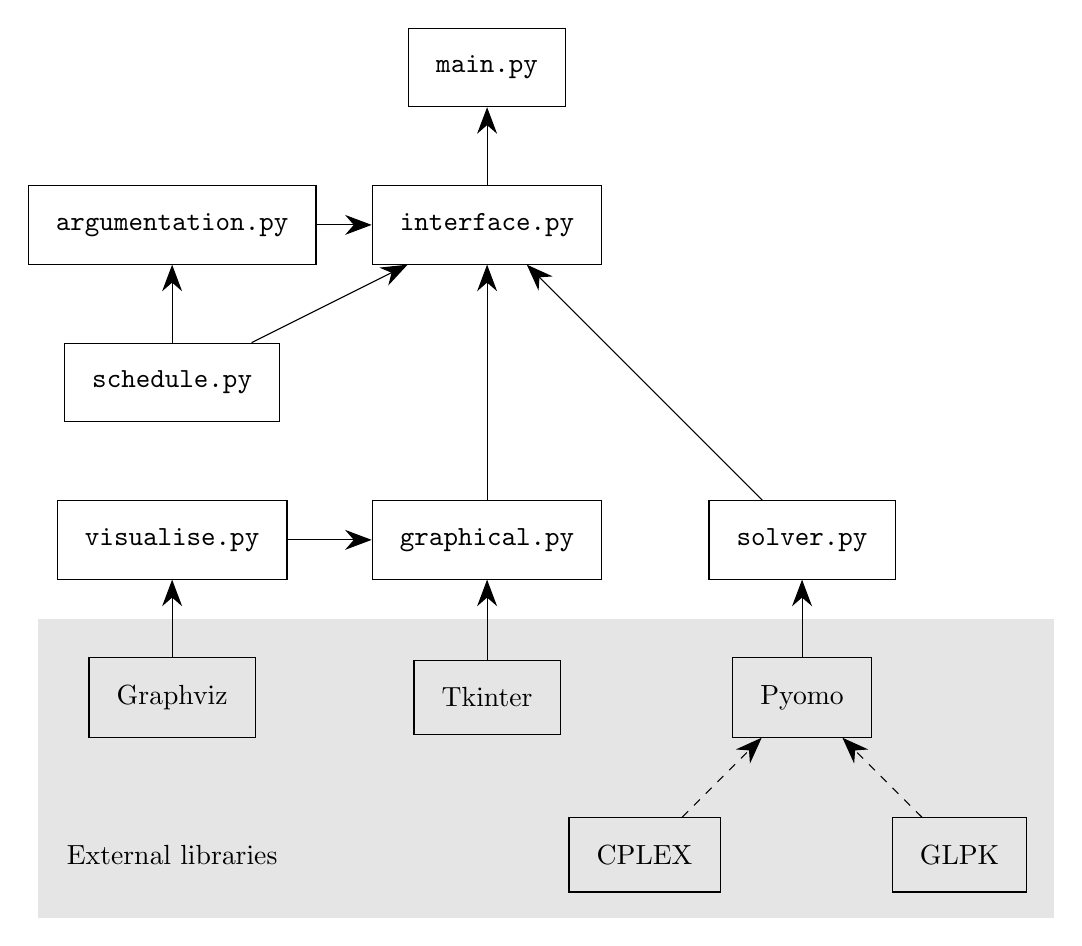
\begin{tikzpicture}
	\fill[fill=black!10](-1.7, -0.8) rectangle (11.2, 3);
	\node at (0, 0){External libraries};

	\node[file](cplex) at (6, 0){CPLEX};
	\node[file](glpk) at (10, 0){GLPK};
	\node[file](graphviz) at (0, 2){Graphviz};
	\node[file](tkinter) at (4, 2){Tkinter};		
	\node[file](pyomo) at (8, 2){Pyomo};
	\node[file](visualise) at (0, 4){\verb|visualise.py|};
	\node[file](graphical) at (4, 4){\verb|graphical.py|};
	\node[file](solver) at (8, 4){\verb|solver.py|};
	\node[file](schedule) at (0, 6){\verb|schedule.py|};
	\node[file](argumentation) at (0, 8){\verb|argumentation.py|};
	\node[file](interface) at (4, 8){\verb|interface.py|};
	\node[file](main) at (4, 10){\verb|main.py|};
	\draw[arrow, dashed](cplex) -- (pyomo);
	\draw[arrow, dashed](glpk) -- (pyomo);
	\draw[arrow](graphviz) -- (visualise);
	\draw[arrow](pyomo) -- (solver);
	\draw[arrow](tkinter) -- (graphical);
	\draw[arrow](visualise) -- (graphical);
	\draw[arrow](graphical) -- (interface);
	\draw[arrow](solver) -- (interface);
	\draw[arrow](argumentation) -- (interface);
	\draw[arrow](schedule) -- (interface);
	\draw[arrow](schedule) -- (argumentation);
	\draw[arrow](interface) -- (main);
\end{tikzpicture}

The above graph illustrates the functional dependency between modules. A solver is required for full functionality of the tool. This could be CPLEX or GLPK.

\section{Algorithms}

\subsection{Notation}

\begin{definition}
	Let $\mathbf{0}^{d_1, ..., d_n}$ be the zero-valued binary tensor. The dimensions may be omitted if clear. Matrix subscripts are extended to $n$ dimensions.
		
	For example:
	\begin{align*}
	\mathbf{0}^{2\times 2}&=
	\begin{bmatrix}
	0&0\\
	0&0\\
	\end{bmatrix}
	\end{align*}
\end{definition}

\begin{definition}
	Let $\incircbin{\neg}$ be the element-wise logical negation operator over a tensor.
	
	For example:
	\begin{align*}
		\incircbin{\neg}
		\begin{bmatrix}
		1&0\\
		0&1\\
		\end{bmatrix}&=
		\begin{bmatrix}
			0&1\\
			1&0\\
		\end{bmatrix}
	\end{align*}
\end{definition}

\begin{definition}
	Let $\incircbin{\land}$ be the element-wise logical and operator over tensors.
	
	For example:
	\begin{align*}
	\begin{bmatrix}
	0&0\\
	1&1\\
	\end{bmatrix}
	\incircbin{\land}
	\begin{bmatrix}
	0&1\\
	0&1\\
	\end{bmatrix}
	&=
	\begin{bmatrix}
	0&0\\
	0&1\\
	\end{bmatrix}
	\end{align*}
\end{definition}

\begin{definition}
	Let $\incircbin{\lor}$ be the element-wise logical or operator over tensors.
	
	For example:
	\begin{align*}
	\begin{bmatrix}
	0&0\\
	1&1\\
	\end{bmatrix}
	\incircbin{\lor}
	\begin{bmatrix}
	0&1\\
	0&1\\
	\end{bmatrix}
	&=
	\begin{bmatrix}
	0&1\\
	1&1\\
	\end{bmatrix}
	\end{align*}
\end{definition}

\subsection{Framework Construction}

The AAFs are constructed using the definitions in paper.\cite{aes} The definitions are reprinted below. Take arbitrary $i_1,i_2\in\mathcal{M}$ and $j_1,j_2\in\mathcal{J}$.

\begin{definition}
	The feasiblity framework $\rightsquigarrow_F$ is defined such that $\langle i_1,j_1\rangle\rightsquigarrow_F\langle i_2,j_2\rangle$ iff $i_1\neq i_2\land j_1=j_2$.
\end{definition}

\begin{definition}
	The efficiency framework $\rightsquigarrow_S$ is defined such that $\langle i_1,j_1\rangle\rightsquigarrow_S\langle i_2,j_2\rangle\land\neg\text{SEP}(i_1,i_2,j_1)\lor\text{PEP}(i_1,i_2,j_1,j_2)$ where:
	\begin{itemize}
		\item Single exchange property: $\text{SEP}(i_1,i_2,j_1)$ iff $C_{i_1}=C_{\max}\land x_{i_1,j_1}=1\land C_{i_1}>C_{i_2}+p_{j_1}$
		\item Pair-wise exchange property: $\text{PEP}(i_1,i_2,j_1,j_2)$ iff $C_{i_1}=C_{\max}\land x_{i_1,j_1}=1\land x_{i_2,j_2}=1\land i_1\neq i_2\land j_1\neq j_2\land p_{j_1}>p_{j_2}\land C_{i_1}+p_{j_2}>C_{i_2}+p_{j_1}$.
	\end{itemize}
\end{definition}

\begin{definition}
	The fixed user decision framework $\rightsquigarrow_D$ is defined such that $\langle i_1,j_1\rangle\rightsquigarrow_S\langle i_2,j_2\rangle\land\neg\text{DP}^+(i_1,i_2,j_1,j_2)\lor\text{DP}^-(i_1,i_2,j_1,j_2)$ where:
	\begin{itemize}
		\item Positive decision property: $\text{DP}^+(i_1,i_2,j_1,j_2)$ iff $\langle i_2, j_2\rangle\in D^+$
		\item Negative decision property: $\text{DP}^-(i_1,i_2,j_1,j_2)$ iff $\langle i_1, j_1\rangle\in D^-\land i_1=i_2\land j_1=j_2$.
	\end{itemize}
\end{definition}

\begin{algorithm}[h!]
	\begin{algorithmic}[1]
		\Function{Construct-Feasibilty}{$m$, $n$}
			\State $\rightsquigarrow_F$ $\gets$ $\mathbf{0}^{(m\times n)^2}$
			\For{$j\in\mathcal{J}$}
				\For{$i_1\in\mathcal{M}$}
					\For{$i_2\in\mathcal{M}$}
						\If{$i_1\neq i_2$}
							\State ${\rightsquigarrow_F}_{i_1,j,i_2,j}$ $\gets$ 1
						\EndIf
					\EndFor
				\EndFor
			\EndFor
			\State \Return $\rightsquigarrow_F$
		\EndFunction
	\end{algorithmic}
\end{algorithm}

$\rightsquigarrow_F$ can be constructed trivally in a dense data structure in $\mathcal{O}(m^2n^2)$ computational complexity. because of the complexity of zero-initialising $\rightsquigarrow_F$. This can be constructed in $\mathcal{O}(m^2n)$ complexity using a sparse data strucutre, but results in greatly more complicated code.

\begin{algorithm}[h!]
	\begin{algorithmic}[1]
		\Function{Construct-Efficiency}{$m$, $n$, $\mathbf{p}$, $\mathbf{x}$, $\rightsquigarrow_F$}
			\State $\mathbf{C}$ $\gets$ $\mathbf{x}\cdot\mathbf{p}$
			\State $C_{\max}$ $\gets$ $\max(\mathbf{C})$
			\State $\rightsquigarrow_S$ $\gets$ $\rightsquigarrow_F$
			\For{$i_1\in\mathcal{M}$}
				\If{$i_1\neq C_{\max}$}
					\For{$j_1\in\mathcal{J}$}
						\If{$x_{i_1,j_1}=1$}
							\For{$i_2\in\mathcal{M}$}
								\If{$\text{SEP}(i_1,j_1,i_2)$}
									\State ${\rightsquigarrow_S}_{i_1,j_1,i_2,j_1}$ $\gets$ 0
								\EndIf
								\For{$j_2\in\mathcal{J}$}
									\If{$\text{PEP}(i_1,j_1,i_2,j_2)$}
										\State ${\rightsquigarrow_S}_{i_1,j_2,i_2,j_2}$ $\gets$ 1
									\EndIf
								\EndFor
							\EndFor
						\EndIf
					\EndFor
				\EndIf
			\EndFor
			\State \Return $\rightsquigarrow_S$
		\EndFunction
	\end{algorithmic}
\end{algorithm}

The construction of $\rightsquigarrow_S$ is expensive because of the explict for-loops to iterate over the $\mathcal{M}^2\mathcal{J}^2$ space to compute the edges that satisify PEP and to copy $\rightsquigarrow_F$. An optimisation by computing SEP outside of the $j_2$ loop, because PEP is invariant of $j_2$.

\begin{algorithm}[h!]
	\begin{algorithmic}[1]
		\Function{Construct-Efficiency}{$m$, $n$, $D$, $\rightsquigarrow_F$}
			\State $\rightsquigarrow_D$ $\gets$ $\rightsquigarrow_F$
			\For{$\langle i,j\rangle\in D^-$}
				\State ${\rightsquigarrow_S}_{i,j,i,j}$ $\gets$ 1
			\EndFor
			\For{$\langle i_1,j_1\rangle\in D^+$}
				\For{$i_2\in\mathcal{M}$}
					\For{$j_2\in\mathcal{J}$}
						\State ${\rightsquigarrow_D}_{i_2,j_2,i_1,j_1}$ $\gets$ 0				
					\EndFor
				\EndFor
			\EndFor
			\State \Return $\rightsquigarrow_D$
		\EndFunction
	\end{algorithmic}
\end{algorithm}

The construction of $\rightsquigarrow_D$ has $\mathcal{O}(m^2n^2)$ computational complexity. If $D$ is assumed to be satisfible, then $D^+$ has at most $n$ decisions while $D^-$ has at most $m-1)n$ decisions. However, if $D$ is not neccessarly satifible to account for poorly-formulated user problems, so in general $D^+$ and $D^-$ has at most $mn$ decisions.

\subsection{Stability}

Stability can be computed by checking whether $E$ exists within a all possible stable extensions of some $\langle Args, \rightsquigarrow\rangle$. However, a schedule cannot be reasoned on without understanding whether $E$ may be stable on $\langle Args, \rightsquigarrow\rangle$. Existing solutions require a complication pipeline using answer set solvers. To make the implementation of the tool easier, we adapt the stability computation to schedules into a concise algorithm.

\begin{algorithm}[h!]
	\begin{algorithmic}[1]
		\Function{Explain-Stability}{$\mathbf{x}$, $\rightsquigarrow$,
			 ignoreUnattacked, ignoreConflicts}
			\State unattacked $\gets\incircbin{\neg}$ $\mathbf{x}$
			\State conflicts $\gets\mathbf{0}^{(m\times n)^2}$
			\For{$i\in\mathcal{M}$}
				\For{$j\in\mathcal{J}$}
					\If{$E_{i,j}=1$}
						\State unattacked $\gets$ unattacked $\incircbin{\land}$ $\incircbin{\neg}\rightsquigarrow_{i,j}$
						\State conflicts$_{i,j}$ $\gets$ $\mathbf{x}$ $\incircbin{\land}$ $\rightsquigarrow_{i,j}$ 
					\EndIf
				\EndFor
			\EndFor
			\State unattacked $\gets$ unattacked $\incircbin{\land}$ $\incircbin{\neg}$ ignoreUnattacked
			\State conflicts $\gets$ conflicts $\incircbin{\land}$ $\incircbin{\neg}$ ignoreConflicts
			\State \Return unattacked, conflicts
		\EndFunction
	\end{algorithmic}
\end{algorithm}

The function returns two tensors, \emph{unattacked} encode the unattacked nodes and \emph{conflicts} encode the edges are not conflict-free. \emph{ignoreUnattack} and \emph{ignoreConflicts} represent node and edges to ignore from returned values respectively, which are useful in tailoring explanations to particular constraints. By default, ignoreUnattacked $=\mathbf{0}$ and ignoreConflicts $=\mathbf{0}$. The algorithm has $\mathcal{O}(m^2n^2)$ computational and memory complexity. The function uses $\mathbf{x}$ rather than its equivalent representation $E$ because $\mathbf{x}$ can be manipulated directly from an optimiser in its tensor form unlike $E$. In addition, it is assumed that $E\subseteq Args$ so $Args$ does not need to be a parameter.

\begin{theorem}
	\textsc{Explain-Stability} is correct where $\mathbf{x}\approx E$ under $S$:
	\begin{align*}
		\textsc{Explain-Stability}(\mathbf{x},\rightsquigarrow,\mathbf{0},\mathbf{0})=\langle \mathbf{0},\mathbf{0}\rangle\Leftrightarrow E\text{ is stable on }\langle Args, \rightsquigarrow\rangle
	\end{align*}
\end{theorem}
	
\subsection{Explanation}

\begin{algorithm}[h!]
	\begin{algorithmic}[1]
		\Function{Explain-Schedule}{$m$, $n$, $\mathbf{p}$, $D$, $\mathbf{x}$}
				\State $\rightsquigarrow_F$ $\gets$ \textsc{Construct-Feasibility}($m$, $n$)
				\State $\langle$ unattacked\textsubscript{F}, conflicts\textsubscript{F} $\rangle$ $\gets$ \textsc{Explain-Stability}($\mathbf{x}$, $\rightsquigarrow_F$, $\mathbf{0}$, $\mathbf{0}$)
				\State explanation\textsubscript{F} $\gets$ \textsc{Explain-Feasibility}(unattacked\textsubscript{F}, conflicts\textsubscript{F})

				\State $\rightsquigarrow_S$ $\gets$ \textsc{Construct-Efficiency}($m$, $n$, $\mathbf{p}$, $\mathbf{x}$, $\rightsquigarrow_F$)
				\State $\langle$ unattacked\textsubscript{S}, conflicts\textsubscript{S} $\rangle$ $\gets$ \textsc{Explain-Stability}($\mathbf{x}$, $\rightsquigarrow_S$, unattacked\textsubscript{F}, conflicts\textsubscript{F})
				\State explanation\textsubscript{F} $\gets$ \textsc{Explain-Efficiency}(unattacked\textsubscript{S}, conflicts\textsubscript{S})

				\State $\rightsquigarrow_D$ $\gets$ \textsc{Construct-Satisfaction}($m$, $n$, $\mathbf{x}$, $\rightsquigarrow_F$)
				\State $\langle$ unattacked\textsubscript{D}, conflicts\textsubscript{D} $\rangle$ $\gets$ \textsc{Explain-Stability}($\mathbf{x}$, $\rightsquigarrow_D$, unattacked\textsubscript{F}, conflicts\textsubscript{F})
				\State explanation\textsubscript{F} $\gets$ \textsc{Explain-Satisfaction}(unattacked\textsubscript{D}, conflicts\textsubscript{D})
				
				\State explanation $\gets$ \textsc{Aggregate}(explanation\textsubscript{F}, explanation\textsubscript{S}, explanation\textsubscript{D})
				\State \Return explanation
		\EndFunction
	\end{algorithmic}
\end{algorithm}

	\chapter{Evaluation}

\section{Measures of Success}

The success of the project can be measured by comparing the project results with objectives. We will also review the design choices in constructing the tool. The review will highlight the practical outcomes from using argumentation to explain scheduling.
\linespace
Arguably, the most important outcome of this project is that the tool is functionality correct. This means the tool is required to explain schedules for feasibility, efficiency and satisfaction with respect to user decisions.
\linespace
One objective is to implement an accessible tool. To measure accessibility, we can refer to the tractability complexity from explanations. The length of explanations either in the number of words or characters may be correlated with understandability. In addition, we conduct a survey targeted towards potential users. Because the understandability of explanations are difficult to measure, we will use open-ended questions. To carefully evaluate explanations, one would need to refer to cognitive science, which is beyond the scope of this project. We use a survey to measure the accessibility of our tool. Moreover, we can measure performance to reflect responsiveness and scalability of the tool \cite{foundationimplementation}. This may be achieved by using profiling utilities to measure performance metrics such as execution time and memory consumption. 

\section{Theoretical Results}

We summarise our complexity results from Chapter \ref{implementation}.

\begin{figure}[H]
	\begin{tabular}{lccc}
		\hline
		Algorithm & Computational & Memory & Tractability\\
		\hline
		\textsc{Construct-Feasibility} & $\mathcal{O}(m^2n^2)$ & $\mathcal{O}(m^2n^2)$ &\\
		\textsc{Construct-Efficiency} & $\mathcal{O}(m^2n^2)$ & $\mathcal{O}(m^2n^2)$ &\\
		\textsc{Construct-Satisfaction} & $\mathcal{O}(m^2n)$ & $\mathcal{O}(m^2n^2)$ &\\
		\textsc{Compute-Unattacked} & $\mathcal{O}(m^2n^2)$ & $\mathcal{O}(mn)$ &\\
		\textsc{Compute-Partial-Conflicts} & $\mathcal{O}(mn)$ & $\mathcal{O}(mn)$ &\\
		\textsc{Explain-Stability} & $\mathcal{O}(m^2n^2)$ & $\mathcal{O}(m^2n^2)$ &\\
		\textsc{Explain-Feasibility} & $\mathcal{O}(mn^2)$ & $\mathcal{O}(mn)$ & $\mathcal{O}(mn)$\\
		\textsc{Explain-Efficiency} & $\mathcal{O}(mn^2\log(mn^2))$ & $\mathcal{O}(mn^2)$ & $\mathcal{O}(mn^2)$\\
		\textsc{Explain-Satisfaction} & $\mathcal{O}(mn)$ & $\mathcal{O}(mn)$ & $\mathcal{O}(mn)$\\
		\textsc{Full-Precomputation-Explain} & $\mathcal{O}(m^2n^2\log(mn^2))$ & $\mathcal{O}(m^2n^2)$ & $\mathcal{O}(mn^2)$\\
		\textsc{Partial-Precomputation-Explain} & $\mathcal{O}(m^2n^2\log(mn^2))$ & $\mathcal{O}(mn^2)$ & $\mathcal{O}(mn^2)$\\
		\hline
	\end{tabular}
	\caption{Computational, memory and tractability complexity of algorithms using argumentation}
\end{figure}

Using an naive explanation approach only improves the computational complexity of verifying the feasibility property, from $\mathcal{O}(m^2n^2)$ to $\mathcal{O}(mn)$.

\section{Practical Results} 

The tool's functionality is demonstrated in the user documentation guide in Appendix \ref{userguide}. We will compare different implementation methods and see how fit for purpose our tool is through a survey.

\subsection{Comparison of Explanation Generation Methods}

We will compare two algorithmic approaches to AAF construction with and the naive approach without argumentation. The algorithms are implemented, then profiled for elapsed time and maximum allocated memory. The time and memory are measured with the Python's \texttt{cProfile} and \texttt{memory-profiler} modules respectively. The tool was executed on Department of Computing's virtual machines, with the specification of dual-core CPU at 2GHz with 2GiB RAM.
\linespace
Time comparison:
\begin{itemize}
	\item Elapsed time measurements are noisy.
	\item For less than 100 jobs, all approaches have approximately equal timings.
	\item From profiling, the tool takes 0.4 seconds on average to startup.
	\item Partial precomputation is 3\% faster than full precomputation on average, excluding startup time.
	\item Naive is 18\% faster than partial precomputation on average, excluding startup time.
	\item Both graphs hints at quadratic complexity.
\end{itemize}

Memory comparison:
\begin{itemize}
	\item For less than 40 jobs, all approaches have approximately equal memory usage.
	\item From profiling, the tool uses 52MiB on average to startup.
	\item For a large number of jobs, partial-precomputation is 7 times more efficient than full precomputation excluding startup memory.
	\item Naive and partial-precomputation have less than 1\% memory usage difference.
	\item Both graphs hints at quadratic complexity.
\end{itemize}

\newpage

\begin{figure}[H]
	\centering
	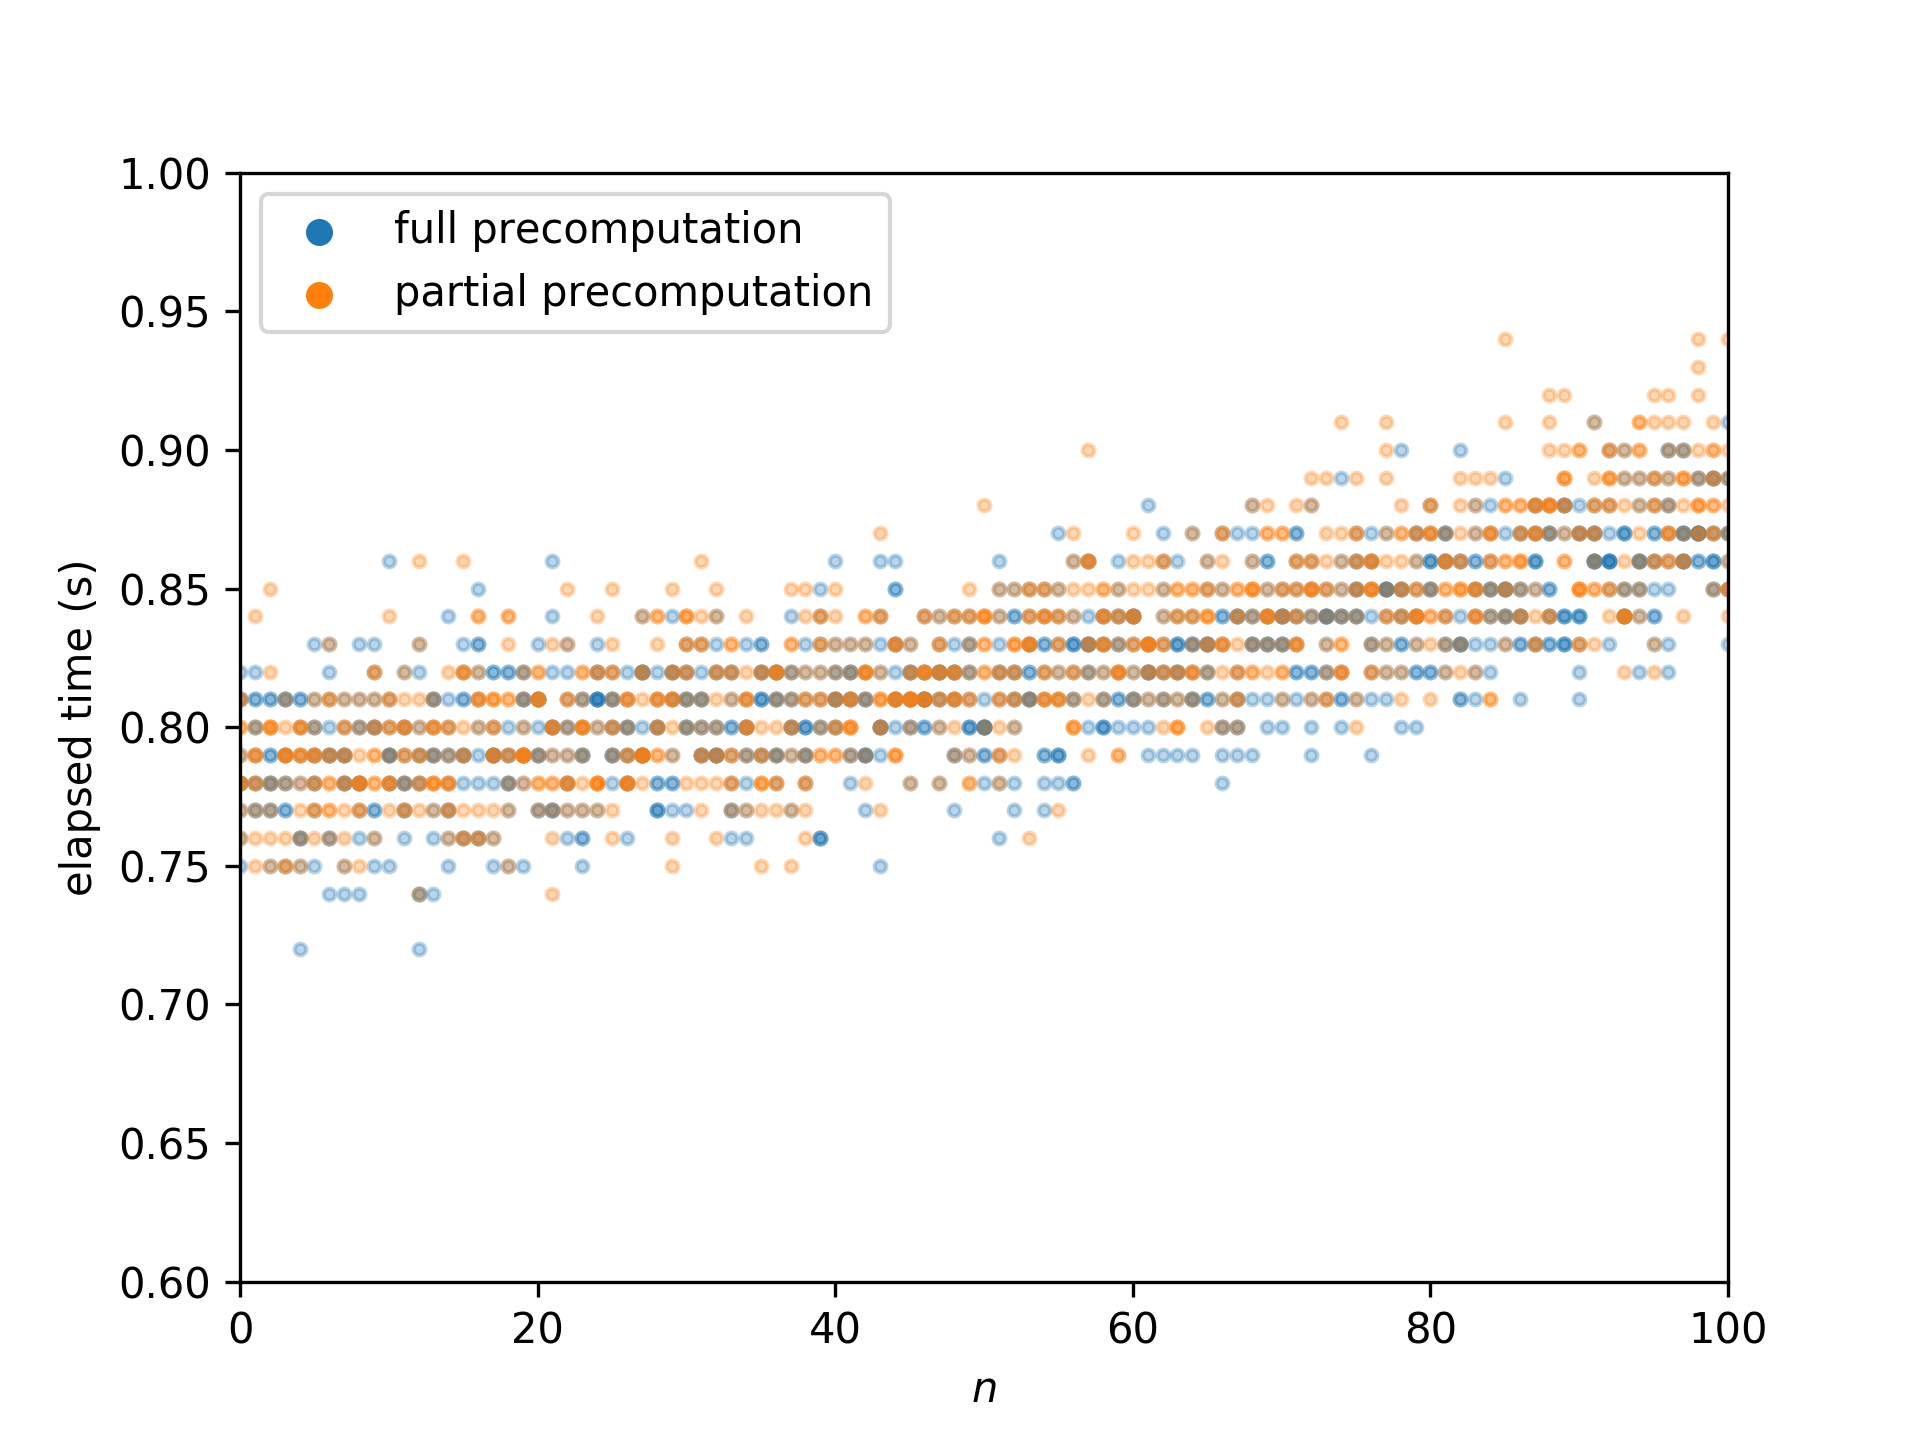
\includegraphics[scale=0.7]{figures/precomputation_cpu_small}
	\caption{Elapsed time comparison where $m=10$ and $0\leq n\leq 100$ with 1000 samples.}
\end{figure}

\begin{figure}[H]
	\centering
	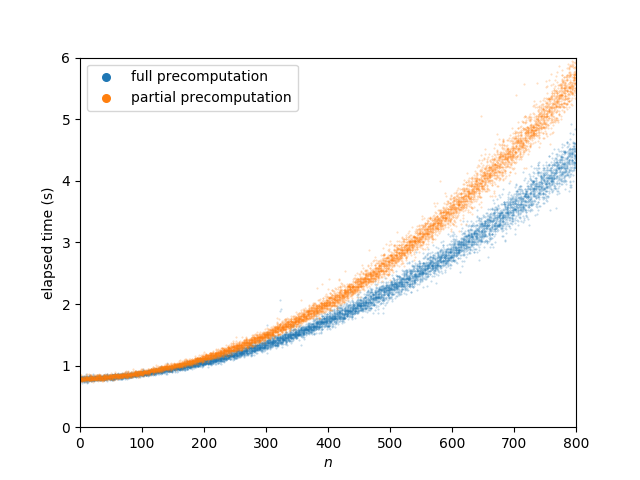
\includegraphics[scale=0.7]{figures/precomputation_cpu_big}
	\caption{Elapsed time comparison where $m=10$ and $0\leq n\leq 800$ with 8000 samples.}
\end{figure}

\begin{figure}[H]
	\centering
	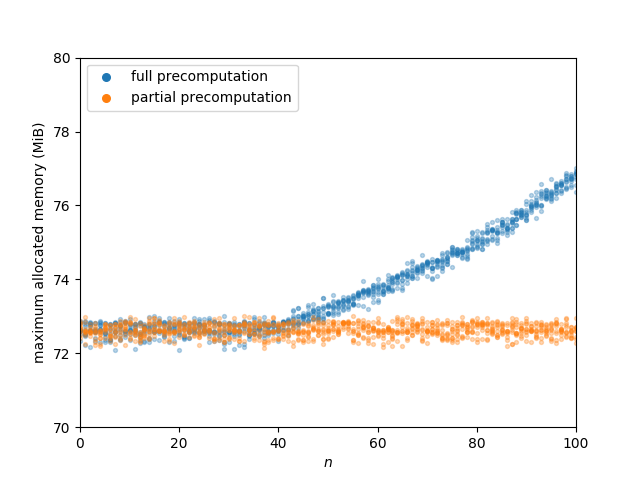
\includegraphics[scale=0.7]{figures/precomputation_memory_small}
	\caption{Maximum allocated memory comparison where $m=10$ and $0\leq n\leq 100$ with 1000 samples.}
\end{figure}

\begin{figure}[H]
	\centering
	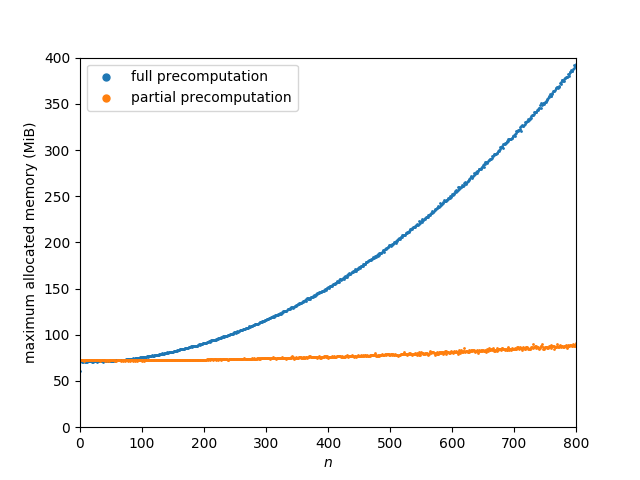
\includegraphics[scale=0.7]{figures/precomputation_memory_big}
	\caption{Maximum allocated memory comparison where $m=10$ and $0\leq n\leq 800$ with 8000 samples.}
\end{figure}

\subsection{Survey}

We conduct a surveys over three sample groups.

\begin{itemize}
	\item \textbf{Group 1}: 10 people who are not given any explanations.
	\item \textbf{Group 2}: 12 people who are given simple explanations generated from the tool, but do not have interactive access to the tool.
	\item \textbf{Group 3}: 7 people who are given interactive access to the tool.
\end{itemize}

In all groups, we used the same questionnaire, which can be found in the appendix. Each question was carefully designed to be completed mentally while exploring concepts in makespan scheduling. We do not ask about feasibility because its validation is trivial. 

\begin{itemize}
	\item Question 1 shows an efficient schedule, but not optimal. The tool does not explain optimality, so users can see there are cases in which the tool may not be helpful.
	\item Question 2 shows a schedule with more machines and jobs, to test whether users can find improvements in a non-trivial schedule. It is possible to optimise the schedule in one single exchange, but this may not be obvious.
	\item Question 3 shows an application of fixed decisions.
	\item Question 4 explores pairs of jobs, which can be modelled using fixed decisions. The question explores how intuition can be formed using additional constraints.
	\item Question 5 explores replanning of a schedule by insertion of a new job. Clearly, trivially inserting a new job does not result in a optimal schedule. It is possible to arrange the schedule in one single exchange before insertion to achieve an optimal updated schedule.
\end{itemize}

Although these five questions do not cover the tool's complete functionality, they cover questions and seek explanations that require intuition, with or without the tool. This is important in assessing how users can operate the tool in non-trivial cases. In this survey, we asked a wide demographic, from GCSE students to graduates, including people who do have little knowledge of computer science or mathematics. 

\subsubsection{Group 1 Results}

\begin{figure}[H]
	\begin{center}
		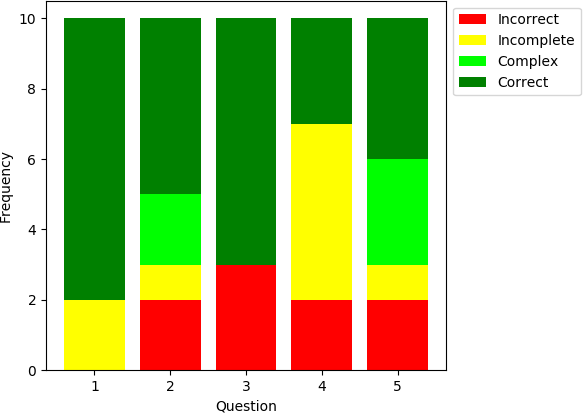
\includegraphics[scale=0.55]{figures/questionnaire_results_group_one}
	\end{center}
	\caption{Aggregated Group 1 results from Section \ref{group1data}}
	\label{group1chart}
\end{figure}

From Figure \ref{group1chart}, we see that the majority of respondents are able to get most questions correct. Some responses are considered complex, when their answers are technically correct, but give more steps than necessary. This may hint that some intuitive ways to optimise a schedule may not minimise the number of job exchanges. This was evident in Question 2 and 5, that has many jobs. We can see in more complex schedules that users give more complex answers. Some responses are considered incomplete, where only the question was partially answered. This was evident in Question 4, where many respondents failed to identity either decision yields an optimal schedule.

\subsubsection{Group 2 Results}

\begin{figure}[H]
	\begin{center}
		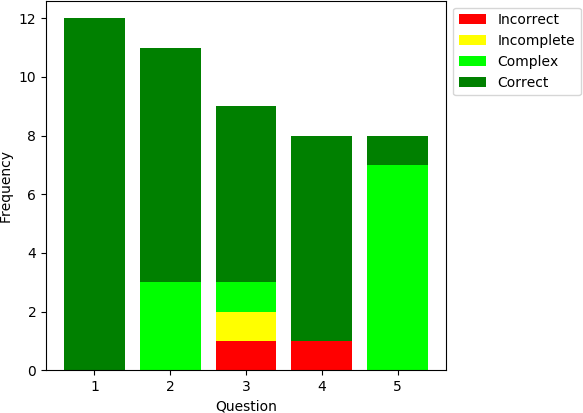
\includegraphics[scale=0.55]{figures/questionnaire_results_group_two}
	\end{center}
	\caption{Aggregated Group 2 results from Section \ref{group2data}}
	\label{group2chart}
\end{figure}

From Figure \ref{group2chart}, we can make the following observations of Group 2 compared to Group 1:
\begin{itemize}
	\item Group 2 respondents performed better than Group 1, and in less time, from 15 minutes 37 seconds to 9 minutes 12 seconds on average, excluding outliers.
	\item Group 1 respondents completed all questions, but there a few Group 2 respondents who did not answer the latter questions. This is illustrated the constant bar heights in Figure \ref{group1chart} and decreasing bar heights in Figure \ref{group2chart}.
	\item When relevant explanations are given in Questions 2 and 5, there are more complex answers in Group 2 than Group 1. The answers suggests that respondents are likely to select the easiest to understand explanation, rather than the simplest optimal schedule. This is significant in Question 5, where many respondents used the first suggestion from the explanation without further intuition.
	\item Question 3 and 4 give situations in which respondents answer which situation results in a more optimal schedule. We can see that explanations significantly improve answers.
	\item In question 1, the explanation given was not relevant, so we would expect answers from Groups 1 and 2 would be similar because the underlying question is the same. From the data, we can see some variance between Groups 1 and 2.
\end{itemize}

\subsubsection{Group 3 Results}

\begin{figure}[H]
	\begin{center}
		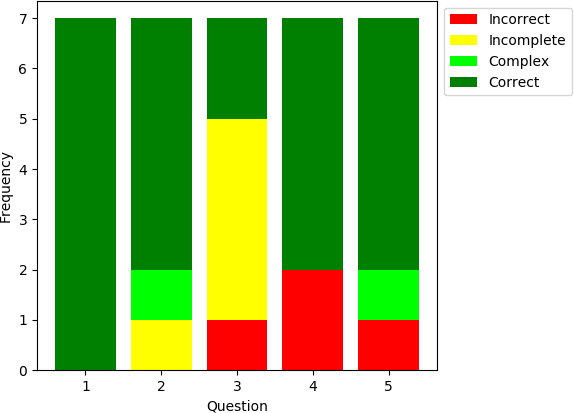
\includegraphics[scale=0.55]{figures/questionnaire_results_group_three}
	\end{center}
	\caption{Aggregated Group 3 results from Section \ref{group3data}}
	\label{group3chart}
\end{figure}

\begin{itemize}
	\item Group 3 respondents took the longest to answer the questions, with 18 minutes and 27 seconds, excluding outliers. Users spent time understanding how to use the tool. To give a more fair comparison of time, users should not been able to start the questionnaire while reading the user guide.
	\item From question 3, many respondents said to simply move jobs to satisfy negative fixed decisions, without concern of the schedule's optimality. This suggests that users took the suggestions from the took too literally. As many users suggested local changes, many answers were considered incompletes.
\end{itemize}

\subsubsection{Summary}

\begin{figure}[H]
	\begin{center}
		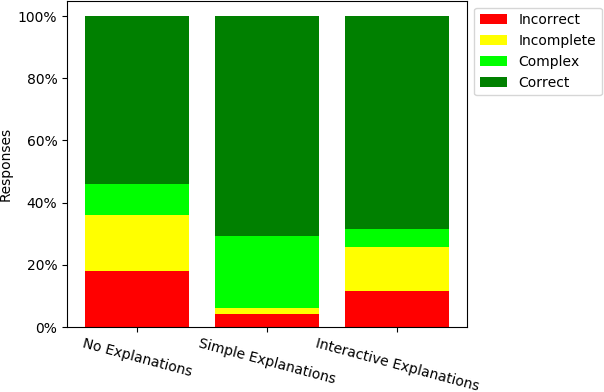
\includegraphics[scale=0.55]{figures/questionnaire_results_summary}
	\end{center}
	\caption{Aggregated results from Figures \ref{group1chart}, \ref{group2chart}, and \ref{group3chart}}
	\label{summarychart}
\end{figure}

\begin{itemize}
	\item Group 1 has the worst performance.
	\item Group 2 has the best performance, but many answers use are long and complex, often using the first obvious solution.
	\item Group 3 has the median performance, with many incomplete answers, using only one iteration of the tool.
\end{itemize}

\subsection{Feedback}

During development of the tool and questionnaires, I asked my colleagues and friends for feedback about the tool.

\begin{itemize}
	\item In early versions of the tool, the GUI did not arrange textboxes and buttons into groups such as problem, schedule and explanation. Instead, all buttons and their functionality were exposed as an menu. This was confusing to new users because it was not evident which textboxes were input or output.
	\item The paper \cite{aes} represented machine job pair assignments as a pairs of integer indices. The tool internally uses indices to compute explanations, however exposing both machines and job as integer indices was confusing. Therefore, jobs are now represented alphabetically.
	\item The tool uses regular expressions to validate user input. Many users complained about the strict validation errors. We solve this by pre-processing the input by correcting missing or surplus white-space.
\end{itemize}
	
	\begin{appendices}
		\chapter{User Guide}

The user guide is a tutorial for non-technical users to learn how to use the tool. The tool has been extensively tested on Linux, the tool has full functionality on Linux and basic functionality on Windows.

\section{Installation}

The tool has the following required dependencies:

\begin{itemize}
	\item Python 3
	\item Tkinter
	\item NumPy
	\item Matplotlib
	\item Pillow
\end{itemize}

Tkinter is the default GUI package for Python and Matplotlib depends on NumPy so Tkinter and Matplotlib do not need to be installed explicitly. The tool has the following optional dependencies:

\begin{itemize}
	\item Pyomo
	\item An optimiser, either CPLEX or GLPK
\end{itemize}

The optional dependencies are used to optimise schedules, these are not strictly required as users can input their own schedules. GLPK is recommended because of its licence and open-source development. The repository is found at \texttt{gitlab.doc.ic.ac.uk/mtl115/aes}. Please refer to the package's websites for troubleshooting. Alternatively, contact the author for assistance.

\subsection{Linux Installation}

The tool was tested on Ubuntu 18.04.1. Python is pre-installed so the following packages can be installed as below:
\begin{verbatim}
apt install python3-pip
apt install python-glpk
apt install glpk-utils
pip3 install matplotlib
pip3 install pillow
pip3 install pyomo
\end{verbatim}

\subsection{Windows Installation}

The tool was tested on Windows 10. First, download Python from the official website, then setup the path environment variable so \texttt{python} can be executed on the command prompt. Afterwards, install the required dependencies as below: 

\begin{verbatim}
python -m pip install matplotlib
python -m pip install pillow
python -m pip install pyomo
\end{verbatim}

\section{Usage}

\subsection{Getting Started}

\begin{figure}[H]
	\centering
	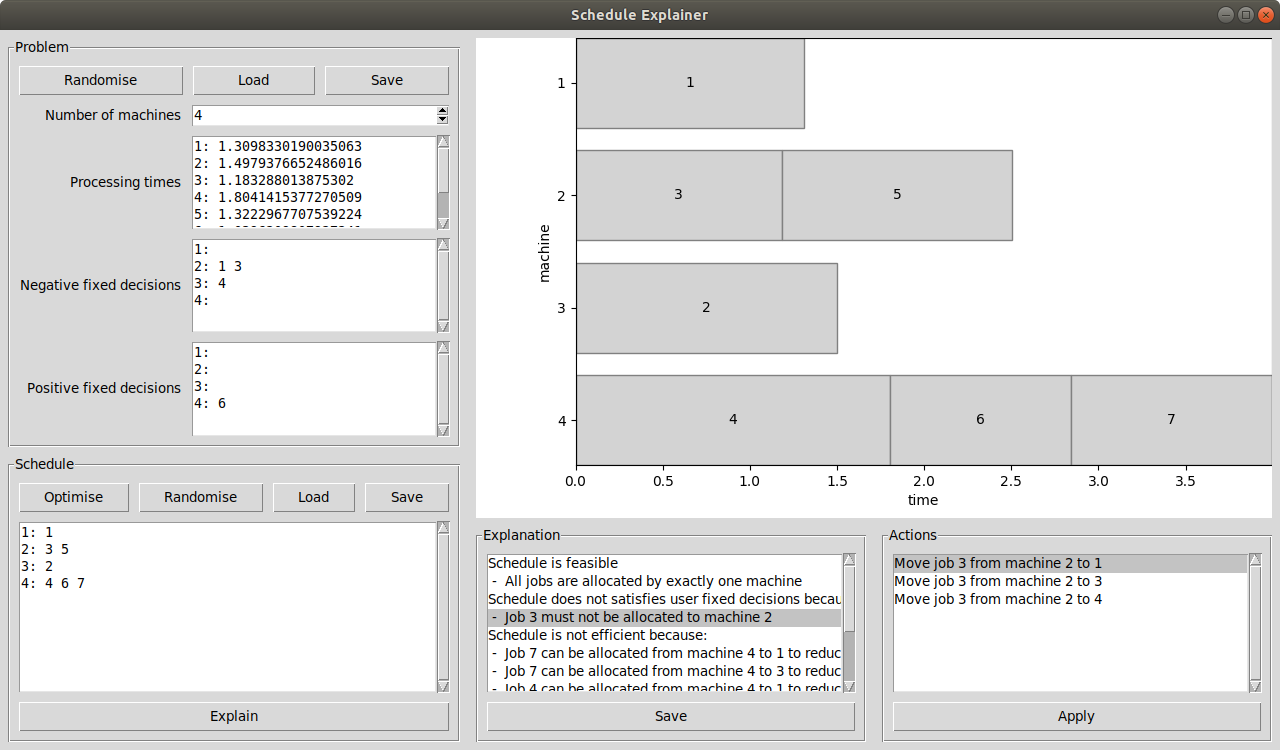
\includegraphics[width=\linewidth]{figures/tool_gui.png}
	\caption{Tool GUI}
\end{figure}

To start the tool, run \texttt{python3 main.py -g} on Linux or \texttt{python main.py -g} on Windows in the \texttt{src} directory supplied in the repository.
\linespace
The makespan problem consists of the number of machines and job processing times. The tutorial will use a hospital setting, where nurses and patients are represented as machines and jobs respectively. Consider the following example where there are two nurses, Alice and Bob. and two patients, Charlie and Dave. Charlie's and Dave's appointment takes 15 and 10 minutes respectively. To enter the example in the tool, nurses and patients are indexed. Hence, A represents Alice, B represents Bob for nurses and 1 represents Charlie and 2 represents Dave for patients. Numbers are used to index machines and letters are used to index jobs. The problem is to minimise the total completion time, which intuitively is the longest time any nurse has to work.

\begin{figure}[H]
	\centering
	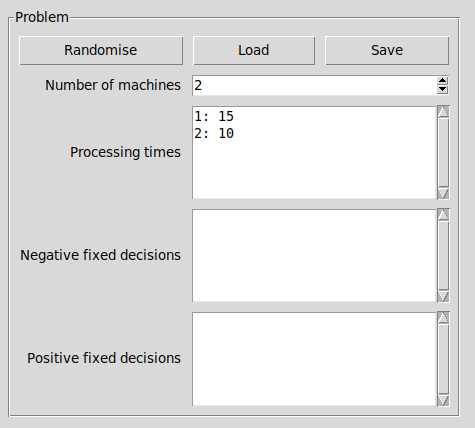
\includegraphics[scale=0.5]{figures/tool_problem.png}
	\caption{Example problem input}
\end{figure}

Each line in the processing time textbox represents one job. The first line can be interpreted as: job A has processing time of 15 units, with following lines having similar interpretations. Negative fixed decisions represent jobs that cannot be assigned to machines. Positive fixed decisions represents jobs that much be assigned to a machine. Note that for all multi-line inputs, each line ends with a new line character.

\begin{figure}[H]
	\centering
	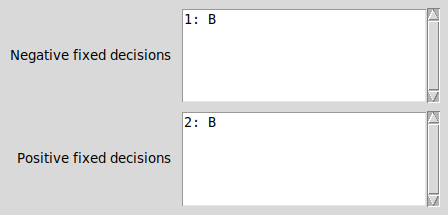
\includegraphics[scale=0.5]{figures/tool_fd.png}
	\caption{Example fixed decisions input}
\end{figure}

Each line in each fixed decisions textbox represents one decision. The first line of negative fixed decisions can be interpreted as: machine 1 cannot be allocated to job B. The first line of positive fixed decisions can be interpreted as: machine 2 cannot be allocated to job B. In context of the example, this means Alice cannot be with Dave and Bob must be with Dave.

\begin{figure}[H]
	\centering
	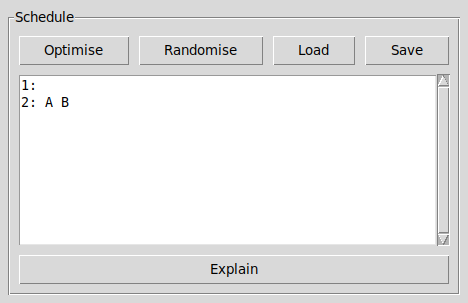
\includegraphics[scale=0.5]{figures/tool_schedule.png}
	\caption{Example schedule input}
\end{figure}

After defining the makespan problem, enter the above schedule. The schedule can be interpreted as: machine 1 has no allocated jobs; machine 2 have two allocated jobs, A and B. The \texttt{Optimise} button finds the optimal schedule using a solver, which is by default GLPK. To specify a solver, starting the tool with \texttt{python3 main.py -g -S SOLVER\_NAME} where \texttt{SOLVER\_NAME} is GLPK or CPLEX, for instance. Note that for large problems, optimisation may take a long time, so a solver time limit can be enforced by starting the tool with \texttt{python3 main.py -g -t TIME\_LIMIT} where \texttt{TIME\_LIMIT} is in seconds. The \texttt{Randomize} button generates some feasible schedule, which may violate fixed decisions. To explain the schedule, click the \texttt{Explain} button. 

\begin{figure}[H]
	\centering
	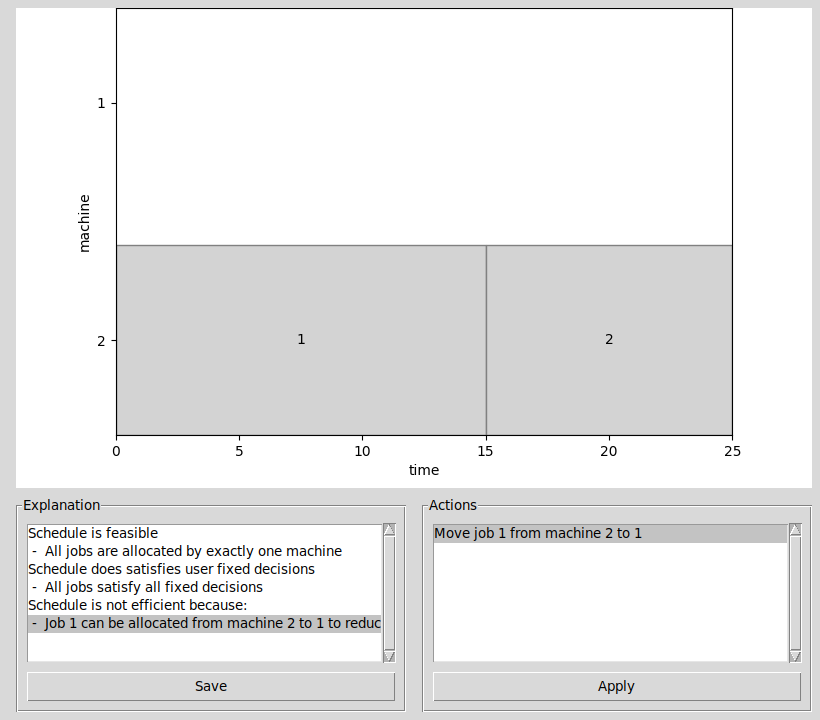
\includegraphics[width=\linewidth]{figures/tool_explain.png}
	\caption{Example explanation output}
\end{figure}

The explanation reasons on three concepts: feasibility, satisfaction of fixed decisions and efficiency. Feasibility ensures that each job is allocated once. Satisfaction of fixed decisions ensures the schedule does not violate negative and positive fixed decisions specified in the problem. Efficiency regards suggestions to improve the total completion time. To improve the schedule, select a line in the explanation listbox to address, then select a line in the actions listbox. An line of explanation may have many different approaches to address the problem or schedule. Click on the \texttt{Apply} button to improve the schedule.

\begin{figure}[H]
	\centering
	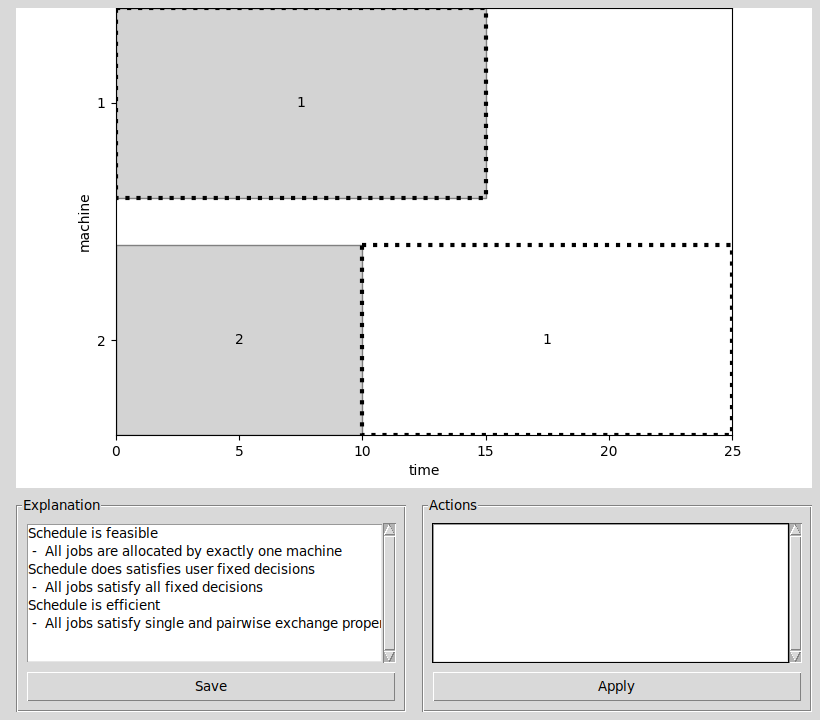
\includegraphics[width=\linewidth]{figures/tool_improve.png}
	\caption{Example explanation output}
\end{figure}

The example schedule only required one action to make the schedule efficient. However, many iterative actions may be required to reach an efficiency schedule. No further actions show that the schedule is feasible, satisfies fixed decisions and is efficient. The dot-highlighted boxes in the cascade chart illustrate newly and removed allocations compared to before the applying the action.

\subsection{Command Line Examples}

\subsubsection{Help Command}

\begin{verbatim}
> python3 main.py -h
usage: main.py [-h] [-g] [-e] [-p PROBLEM | -r [M]]
    [-O | -s SCHEDULE | -R] [-o OUTPUT] [--partial | --naive]
    [-t TIME_LIMIT] [-S SOLVER_NAME]

Explains makespan schedules using abstract argumentation
frameworks

optional arguments:
-h, --help            show this help message and exit
-g, --graphical       displays graphical user interface
-e, --explain         generate explanation
-p PROBLEM, --problem PROBLEM
-r [M], --random_problem [M]
    creates random problem with jobs and fixed decisions
    where M is the number of machines
-O, --optimise        uses SOLVER_NAME to find most efficient
schedule
-s SCHEDULE, --schedule SCHEDULE
-R, --random_schedule
-o OUTPUT, --output OUTPUT
    output filename for selected problem, schedule or
    explanation
--partial             use partial framework construction to
favour memory over CPU
--naive               do not use argumentation
-t TIME_LIMIT, --time_limit TIME_LIMIT
    maximum time for optimisation in seconds, use negative
    time_limit for infinite limit, default is unlimited
time
-S SOLVER_NAME, --solver SOLVER_NAME
    optimisation solver for schedule, default is 'glpk'
\end{verbatim}

\subsubsection{Random problem}

\begin{verbatim}
> python3 main.py -r
4;
A: 1.822
B: 2.994
C: 6.444
D: 2.578
E: 2.386
;
1: B
2: A
3: D
4: B
;
1: 
2: B
3: C
4:
\end{verbatim}

Formally, this represents $m=4$, $n=5$, $\mathbf{p}=\begin{bmatrix}
	1.822&2.994&6.444&2.578&2.386
\end{bmatrix}^T$, $D^-=\{\pair{1}{2},\pair{2}{1},\pair{3}{4},\pair{4}{2}\}$ and $D^+=\{\pair{2}{2}, \pair{3}{3}\}$.

\subsubsection{Random schedule given previous problem}

\begin{verbatim}
> python3 main.py -p example.problem -R
1: A
2: B C E
3: D
4: 
\end{verbatim}

Formally, this represents $\mathbf{x}=\begin{bmatrix}
	1&0&0&0&0\\
	0&1&1&0&1\\
	0&0&0&1&0\\
	0&0&0&0&0\\
\end{bmatrix}$

\subsubsection{Explantation given previous problem and schedule}

\begin{verbatim}
> python3 main.py -p example.problem -s example.schedule -e
Schedule is feasible
-  All jobs are allocated by exactly one machine
Schedule does not satisfies user fixed decisions because:
-  Job C must be allocated to machine 3
-  Job D must not be allocated to machine 3
Schedule is not efficient because:
-  Job C can be allocated from machine 2 to 4 to reduce by 5.38
-  Jobs C and D can be swapped with machines 2 and 3 to reduce by 3.87
-  Job C can be allocated from machine 2 to 1 to reduce by 3.56
-  Job C can be allocated from machine 2 to 3 to reduce by 2.8
-  Job E can be allocated from machine 2 to 1 to reduce by 2.39
-  Job E can be allocated from machine 2 to 3 to reduce by 2.39
-  Job E can be allocated from machine 2 to 4 to reduce by 2.39
\end{verbatim}

\section{Known Limitations}

\begin{itemize}
	\item Holding down space for a button that requires significant computation results in permanent depressed visual of the button. This is a issue with Tkinter.
\end{itemize}
	\end{appendices}

	\cleardoublepage
	\bibliography{bibliography}
	\addcontentsline{toc}{chapter}{Bibliography}
	\bibliographystyle{ieeetr}
\end{document}